% Horizontal stacked bar chart: per-query CPU latency
% BM25-Def: BM25=45, SLM=2800  (total 2845ms)
% HALO:     BM25=45, Dense=38, RRF=5, Reranker=380, SLM=2800 (total 3268ms)
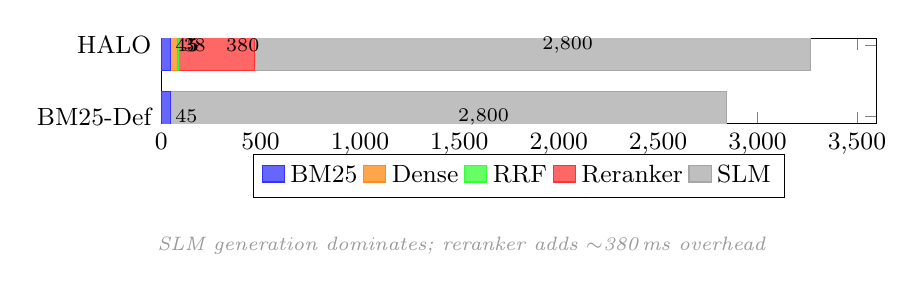
\begin{tikzpicture}
\begin{axis}[
  compat=1.18,
  xbar stacked,
  bar width=18pt,
  width=0.88\textwidth,
  height=0.22\textwidth,
  xmin=0, xmax=3600,
  xlabel={Latency (ms)},
  xlabel style={font=\small},
  x tick label style={font=\small},
  y tick label style={font=\small},
  ytick={1,2},
  yticklabels={BM25-Def, HALO},
  nodes near coords,
  nodes near coords align={horizontal},
  every node near coord/.style={font=\scriptsize},
  legend style={at={(0.5,-0.35)}, anchor=north, font=\small,
                legend columns=5},
  legend cell align=left,
]

% BM25 segment (blue)
\addplot[fill=blue!60, draw=blue!80] coordinates {(45,1) (45,2)};
\addlegendentry{BM25}

% Dense segment (orange) — 0 for BM25-Def, 38 for HALO
\addplot[fill=orange!70, draw=orange!90] coordinates {(0,1) (38,2)};
\addlegendentry{Dense}

% RRF segment (green) — 0 for BM25-Def, 5 for HALO
\addplot[fill=green!60, draw=green!80] coordinates {(0,1) (5,2)};
\addlegendentry{RRF}

% Reranker segment (red) — 0 for BM25-Def, 380 for HALO
\addplot[fill=red!60, draw=red!80] coordinates {(0,1) (380,2)};
\addlegendentry{Reranker}

% SLM segment (gray)
\addplot[fill=gray!50, draw=gray!70] coordinates {(2800,1) (2800,2)};
\addlegendentry{SLM}

\end{axis}

% Annotation note below the chart
\node[font=\scriptsize\itshape, text=gray!80, anchor=north]
  at (current bounding box.south)
  [yshift=-0.25cm]
  {SLM generation dominates; reranker adds ${\sim}$380\,ms overhead};

\end{tikzpicture}
